% Options for packages loaded elsewhere
\PassOptionsToPackage{unicode}{hyperref}
\PassOptionsToPackage{hyphens}{url}
%
\documentclass[
  letterpaper,
  ignorenonframetext,
  aspectratio=43,
  handout,
  12pt]{beamer}
\usepackage{pgfpages}
\setbeamertemplate{caption}[numbered]
\setbeamertemplate{caption label separator}{: }
\setbeamercolor{caption name}{fg=normal text.fg}
\beamertemplatenavigationsymbolsempty
% Prevent slide breaks in the middle of a paragraph
\widowpenalties 1 10000
\raggedbottom
\setbeamertemplate{part page}{
  \centering
  \begin{beamercolorbox}[sep=16pt,center]{part title}
    \usebeamerfont{part title}\insertpart\par
  \end{beamercolorbox}
}
\setbeamertemplate{section page}{
  \centering
  \begin{beamercolorbox}[sep=12pt,center]{part title}
    \usebeamerfont{section title}\insertsection\par
  \end{beamercolorbox}
}
\setbeamertemplate{subsection page}{
  \centering
  \begin{beamercolorbox}[sep=8pt,center]{part title}
    \usebeamerfont{subsection title}\insertsubsection\par
  \end{beamercolorbox}
}
\AtBeginPart{
  \frame{\partpage}
}
\AtBeginSection{
  \ifbibliography
  \else
    \frame{\sectionpage}
  \fi
}
\AtBeginSubsection{
  \frame{\subsectionpage}
}
\usepackage{amsmath,amssymb}
\usepackage{lmodern}
\usepackage{iftex}
\ifPDFTeX
  \usepackage[T1]{fontenc}
  \usepackage[utf8]{inputenc}
  \usepackage{textcomp} % provide euro and other symbols
\else % if luatex or xetex
  \usepackage{unicode-math}
  \defaultfontfeatures{Scale=MatchLowercase}
  \defaultfontfeatures[\rmfamily]{Ligatures=TeX,Scale=1}
\fi
\usetheme[]{metropolis}
% Use upquote if available, for straight quotes in verbatim environments
\IfFileExists{upquote.sty}{\usepackage{upquote}}{}
\IfFileExists{microtype.sty}{% use microtype if available
  \usepackage[]{microtype}
  \UseMicrotypeSet[protrusion]{basicmath} % disable protrusion for tt fonts
}{}
\makeatletter
\@ifundefined{KOMAClassName}{% if non-KOMA class
  \IfFileExists{parskip.sty}{%
    \usepackage{parskip}
  }{% else
    \setlength{\parindent}{0pt}
    \setlength{\parskip}{6pt plus 2pt minus 1pt}}
}{% if KOMA class
  \KOMAoptions{parskip=half}}
\makeatother
\usepackage{xcolor}
\IfFileExists{xurl.sty}{\usepackage{xurl}}{} % add URL line breaks if available
\IfFileExists{bookmark.sty}{\usepackage{bookmark}}{\usepackage{hyperref}}
\hypersetup{
  hidelinks,
  pdfcreator={LaTeX via pandoc}}
\urlstyle{same} % disable monospaced font for URLs
\newif\ifbibliography
\usepackage{graphicx}
\makeatletter
\def\maxwidth{\ifdim\Gin@nat@width>\linewidth\linewidth\else\Gin@nat@width\fi}
\def\maxheight{\ifdim\Gin@nat@height>\textheight\textheight\else\Gin@nat@height\fi}
\makeatother
% Scale images if necessary, so that they will not overflow the page
% margins by default, and it is still possible to overwrite the defaults
% using explicit options in \includegraphics[width, height, ...]{}
\setkeys{Gin}{width=\maxwidth,height=\maxheight,keepaspectratio}
% Set default figure placement to htbp
\makeatletter
\def\fps@figure{htbp}
\makeatother
% Make links footnotes instead of hotlinks:
\DeclareRobustCommand{\href}[2]{#2\footnote{\url{#1}}}
\setlength{\emergencystretch}{3em} % prevent overfull lines
\providecommand{\tightlist}{%
  \setlength{\itemsep}{0pt}\setlength{\parskip}{0pt}}
\setcounter{secnumdepth}{-\maxdimen} % remove section numbering
\usepackage{pgfpages}
\pgfpagesuselayout{2 on 1}
\providecommand{\tightlist}{%
\setlength{\itemsep}{0pt}\setlength{\parskip}{0pt}}
\makeatletter
\makeatother
\let\Oldincludegraphics\includegraphics
\renewcommand{\includegraphics}[2][]{\Oldincludegraphics[width=\textwidth,height=0.7\textheight,keepaspectratio]{#2}}
\ifLuaTeX
  \usepackage{selnolig}  % disable illegal ligatures
\fi

\author{}
\date{}

\begin{document}

\begin{frame}{Theory of Elasticity}
\protect\hypertarget{theory-of-elasticity}{}
Dr.~Nicholas Smith

Wichita State University, Department of Aerospace Engineering October 5,
2021
\end{frame}

\begin{frame}{upcoming schedule}
\protect\hypertarget{upcoming-schedule}{}
\begin{itemize}
\tightlist
\item
  Oct 5 - Strain Energy
\item
  Oct 7 - Exam 2 Review
\item
  Oct 8 - Homework 4 Self-grade Due, Homework 5 Due
\item
  (Oct 12) - Fall Break (No Class)
\item
  Oct 14 - Exam 2
\item
  Oct 19 - Strain Energy
\end{itemize}
\end{frame}

\begin{frame}{outline}
\protect\hypertarget{outline}{}
\begin{itemize}
\tightlist
\item
  strain energy
\item
  uniqueness of elasticity problems
\item
  group problems
\end{itemize}
\end{frame}

\hypertarget{strain-energy}{%
\section{strain energy}\label{strain-energy}}

\begin{frame}{strain energy}
\protect\hypertarget{strain-energy-1}{}
\begin{itemize}
\tightlist
\item
  Work done by surface and body forces is stored as \emph{strain energy}
\item
  In an elastic body, this is completely recoverable
\item
  In one dimension, this is similar to a linear spring
\end{itemize}
\end{frame}

\begin{frame}{strain energy}
\protect\hypertarget{strain-energy-2}{}
\begin{columns}[T]
\begin{column}{0.5\textwidth}
\begin{itemize}
\tightlist
\item
  The strain energy must be equal to the net work done
\item
  Recall ``work'' is force times displacement (force in direction of
  displacement)
\end{itemize}
\end{column}

\begin{column}{0.5\textwidth}
\begin{figure}
\centering
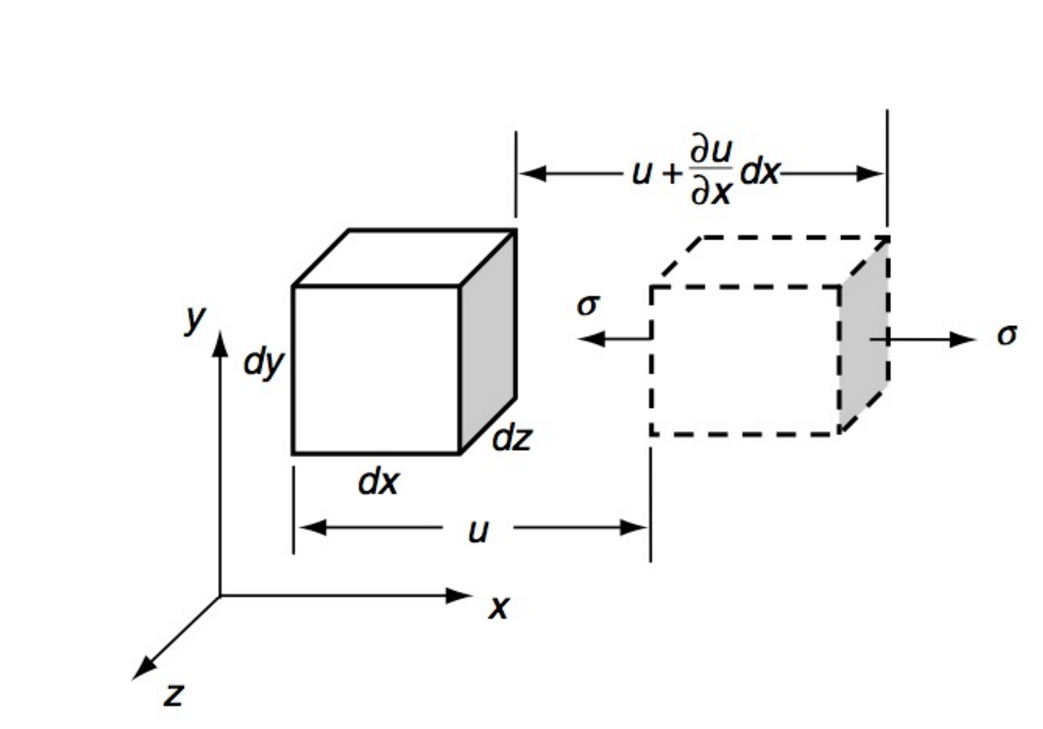
\includegraphics{../images/work.PNG}
\caption{work done}
\end{figure}
\end{column}
\end{columns}
\end{frame}

\begin{frame}{strain energy}
\protect\hypertarget{strain-energy-3}{}
\begin{itemize}
\tightlist
\item
  In uniaxial tension, the net work can be expressed as
\end{itemize}

\[dU = \int_0^{\sigma_x} \sigma d\left(u + \frac{\partial u}{\partial x}dx\right)dydz - \int_0^{\sigma_x} \sigma du dy dz\]

\begin{itemize}
\tightlist
\item
  Or, simplifying
\end{itemize}

\[dU = \int_0^{\sigma_x} \sigma d\left(\frac{\partial u}{\partial x}dx\right)dydz\]
\end{frame}

\begin{frame}{strain energy}
\protect\hypertarget{strain-energy-4}{}
\begin{itemize}
\tightlist
\item
  We can use strain-displacement and Hooke's Law to say
\end{itemize}

\[\frac{\partial u}{\partial x} = \epsilon_x = \frac{\sigma_x}{E}\]

\begin{itemize}
\tightlist
\item
  Substituting this gives
\end{itemize}

\[dU = \int_0^{\sigma_x} \sigma \frac{d \sigma}{E}dxdydz = \frac{\sigma_x^2}{2E} dx dy dz\]
\end{frame}

\begin{frame}{strain energy}
\protect\hypertarget{strain-energy-5}{}
\begin{itemize}
\tightlist
\item
  We define the \emph{strain energy density} as
\end{itemize}

\[U = \frac{dU}{dx dy dz}\]

\begin{itemize}
\tightlist
\item
  In uni-axial tension, this gives
\end{itemize}

\[U = \frac{\sigma_x^2}{2E} = \frac{E \epsilon_x^2}{2} = \frac{1}{2}\sigma_x \epsilon_x\]
\end{frame}

\begin{frame}{strain energy}
\protect\hypertarget{strain-energy-6}{}
\begin{column}{0.5\textwidth}
\begin{itemize}
\tightlist
\item
  We can also visualize the strain energy graphically as the area under
  the stress-strain curve
\end{itemize}
\end{column}

:::::::::::::: :::::::::::::: \{.columns\} ::: \{.column
width=``50\%''\}\\
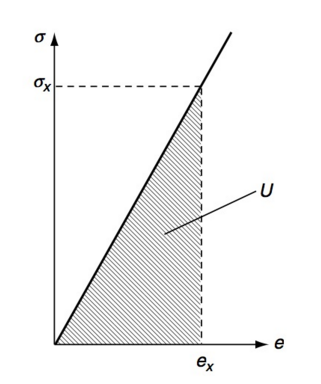
\includegraphics{../images/strain_energy.PNG}

:::
\end{frame}

\begin{frame}{strain energy}
\protect\hypertarget{strain-energy-7}{}
\begin{itemize}
\tightlist
\item
  We can also consider the strain energy due to a uniform shear stress
\end{itemize}

\begin{figure}
\centering
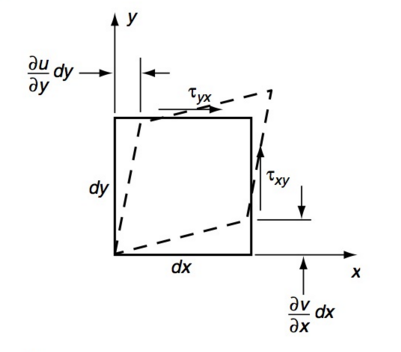
\includegraphics{../images/shear.PNG}
\caption{shear strain energy}
\end{figure}
\end{frame}

\begin{frame}{strain energy}
\protect\hypertarget{strain-energy-8}{}
\begin{itemize}
\tightlist
\item
  Following the same procedure, we find
\end{itemize}

\[dU = \frac{1}{2} \tau_{xy} dydz \left(\frac{\partial v}{\partial x} dx\right) + \frac{1}{2} \tau_{xy} dxdz \left(\frac{\partial u}{\partial y} dy\right) = \frac{1}{2} \tau_{xy} \left(\frac{\partial u}{\partial y} + \frac{\partial v}{\partial x} \right) dx dy dz\]

\begin{itemize}
\tightlist
\item
  And the strain energy density can be expressed as
\end{itemize}

\[U = \frac{1}{2}\tau_{xy}\gamma_{xy} = \frac{\tau_{xy}^2}{2\mu} = \frac{\mu \gamma_{xy}^2}{2}\]
\end{frame}

\begin{frame}{strain energy}
\protect\hypertarget{strain-energy-9}{}
\begin{itemize}
\tightlist
\item
  Using the conservation of energy, we can add the effects from each of
  these loadings to find the total strain energy
\end{itemize}

\[U = \frac{1}{2} \sigma_{ij} \epsilon_{ij}\]

\begin{itemize}
\tightlist
\item
  Note: Although we derived this expression with no body forces, an
  identical solution is found if they are included
\end{itemize}
\end{frame}

\begin{frame}{strain energy}
\protect\hypertarget{strain-energy-10}{}
\begin{itemize}
\tightlist
\item
  To find the total strain energy in a body, we integrate the strain
  energy density over the volume
\end{itemize}

\[U_t = \iiint_V U dx dy dz \]
\end{frame}

\begin{frame}{strain energy}
\protect\hypertarget{strain-energy-11}{}
\begin{itemize}
\tightlist
\item
  As we did before for the uniaxial case, we can write the strain energy
  density in terms of stress or strain only using Hooke's Law
\end{itemize}

\[\begin{aligned}
    U_\epsilon &= \frac{1}{2} \lambda \epsilon_{jj} \epsilon_{kk} + \mu \epsilon_{ij}\epsilon_{ij}\\
    U_\sigma &= \frac{1+\nu}{2E}\sigma_{ij}\sigma_{ij} - \frac{\nu}{2E} \sigma_{jj}\sigma_{kk}
\end{aligned}\]
\end{frame}

\begin{frame}{strain energy}
\protect\hypertarget{strain-energy-12}{}
\begin{itemize}
\tightlist
\item
  If we fully expand both versions, we find that each term is squared
\item
  This means the strain energy must be positive
\end{itemize}
\end{frame}

\begin{frame}{strain energy}
\protect\hypertarget{strain-energy-13}{}
\begin{itemize}
\tightlist
\item
  Another interesting feature we note is that
\end{itemize}

\[\sigma_{ij} = \frac{\partial U_\epsilon}{\partial \epsilon_{ij}}\]

\begin{itemize}
\tightlist
\item
  and
\end{itemize}

\[\epsilon_{ij} = \frac{\partial U_\sigma}{\partial \sigma_{ij}}\]

\begin{itemize}
\tightlist
\item
  These relationships do not depend on stress-strain relations being
  linear, and are often used to derive stresses and strains in
  non-linear materials (\emph{hyperelasticity})
\end{itemize}
\end{frame}

\begin{frame}{strain energy}
\protect\hypertarget{strain-energy-14}{}
\begin{itemize}
\tightlist
\item
  We can further use this relationship to show that
\end{itemize}

\[\begin{aligned}
    \frac{\partial \sigma_{ij}}{\partial \epsilon_{kl}} &= \frac{\partial \sigma_{kl}}{\partial \epsilon_{ij}}\\
    \frac{\partial \epsilon_{ij}}{\partial \sigma_{kl}} &= \frac{\partial \epsilon_{kl}}{\partial \sigma_{ij}}
\end{aligned}\]

\begin{itemize}
\tightlist
\item
  Going to back the general form of Hooke's Law
  (\(\sigma_{ij} = C_{ijkl}\epsilon_{kl}\)), this gives the symmetry
  condition
\end{itemize}

\[C_{ijkl} = C_{klij}\]
\end{frame}

\begin{frame}{strain energy}
\protect\hypertarget{strain-energy-15}{}
\begin{itemize}
\tightlist
\item
  We can separate the strain energy into two parts, the portion caused
  by \emph{volumetric} deformation and the portion caused by
  \emph{distortional} deformation
\end{itemize}

\[U = U_V + U_D\]
\end{frame}

\begin{frame}{strain energy}
\protect\hypertarget{strain-energy-16}{}
\begin{itemize}
\tightlist
\item
  The volumetric portion can be found using the spherical or hydrostatic
  components of stress and strain
\end{itemize}

\[U_V = \frac{1}{2} \tilde{\sigma_{ij}} \tilde{\epsilon_{ij}} = \frac{1}{6}\sigma_{jj} \epsilon_{kk}\]
\end{frame}

\begin{frame}{strain energy}
\protect\hypertarget{strain-energy-17}{}
\begin{itemize}
\tightlist
\item
  The distortional portion can be found as
\end{itemize}

\[U_D = \frac{1}{12\mu} \left[(\sigma_x - \sigma_y)^2 + (\sigma_y - \sigma_z)^2 + (\sigma_z-\sigma_x)^2 + 6(\tau_{xy}^2 + \tau_{yz}^2 + \tau_{zx}^2)\right]\]

\begin{itemize}
\tightlist
\item
  Some failure theories make use of the distortional strain energy
\end{itemize}
\end{frame}

\hypertarget{uniqueness-of-elasticity-problems}{%
\section{uniqueness of elasticity
problems}\label{uniqueness-of-elasticity-problems}}

\begin{frame}{uniqueness}
\protect\hypertarget{uniqueness}{}
\begin{itemize}
\tightlist
\item
  In Chapter 5 we never proved if any solution was unique
\item
  Let us assume that there exist two solutions to a given boundary value
  problem
\item
  The difference of the two solutions is given as
\end{itemize}

\[\begin{aligned}
    \sigma_{ij} &= \sigma_{ij}^{(1)} - \sigma_{ij}^{(2)}\\
    \epsilon_{ij} &= \epsilon_{ij}^{(1)} - \epsilon_{ij}^{(2)}\\
    u_i &= u_i^{(1)} - u_i^{(2)}
\end{aligned}\]
\end{frame}

\begin{frame}{uniqueness}
\protect\hypertarget{uniqueness-1}{}
\begin{itemize}
\tightlist
\item
  Because both solutions will have the same body force, the difference
  solution must satisfy the equilibrium equation
\end{itemize}

\[\sigma_{ij,j} = 0\]

\begin{itemize}
\tightlist
\item
  We also know that the difference must give
\end{itemize}

\[T_i^n = \sigma_{ij}n_j = 0\]

On the traction boundary and

\[u_i = 0\]

On the displacement boundary
\end{frame}

\begin{frame}{uniqueness}
\protect\hypertarget{uniqueness-2}{}
\begin{itemize}
\tightlist
\item
  Using the definition of strain energy, we can write
\end{itemize}

\[\begin{aligned}
    2 \int_V U dV &= \int_V \sigma_{ij} \epsilon_{ij} dV = \int_V \sigma_{ij}(u_{i,j}-\omega_{ij}) dV\\
    &= \int_V \sigma_{ij}u_{i,j} = \int_V (\sigma_{ij}u_i)_{,j} dV - \int_V \sigma_{ij,j}u_i dV\\
    &= \int_S \sigma_{ij}n_j u_i dS - \int_V \sigma_{ij,j}u_i dV
\end{aligned}\]
\end{frame}

\begin{frame}{uniqueness}
\protect\hypertarget{uniqueness-3}{}
\begin{itemize}
\tightlist
\item
  Note that a symmetric matrix times an antisymmetric matrix =0
\item
  We know that \(\sigma_{ij}n_j = 0\) on surfaces where tractions are
  defined and that \(u_i = 0\) on the other surfaces, so the first
  integral goes to zero
\item
  We also know by equilibrium that \(\sigma_{ij,j}\), so the second
  integral will also be 0
\end{itemize}
\end{frame}

\begin{frame}{uniqueness}
\protect\hypertarget{uniqueness-4}{}
\begin{itemize}
\tightlist
\item
  If the strain energy of the difference between two solutions is zero,
  then we know that

  \begin{itemize}
  \tightlist
  \item
    The stress field of the difference is zero
  \item
    The strain field of the difference is zero
  \item
    The displacement field of the difference is zero
  \end{itemize}
\item
  Therefore the two solutions are the same solution, and the solution is
  unique
\end{itemize}
\end{frame}

\hypertarget{group-problems}{%
\section{group problems}\label{group-problems}}

\begin{frame}{uniaxial tension}
\protect\hypertarget{uniaxial-tension}{}
\begin{itemize}
\tightlist
\item
  We can establish bounds on physical constants by recalling that the
  strain energy must always be positive and considering certain states
  of stress
\item
  Uniaxial tension gives the stress state
\end{itemize}

\[\sigma_{ij} = \begin{bmatrix}
    \sigma & 0 & 0 \\
    0 & 0 & 0\\
    0 & 0 & 0
\end{bmatrix}\]

\begin{itemize}
\tightlist
\item
  Find the strain energy and use it to place bounds on the modulus of
  Elasticity, \emph{E}
\end{itemize}
\end{frame}

\begin{frame}{simple shear}
\protect\hypertarget{simple-shear}{}
\begin{itemize}
\tightlist
\item
  If we consider uniform simple shear
\end{itemize}

\[\sigma_{ij} = \begin{bmatrix}
    0 & \tau & 0 \\
    \tau & 0 & 0\\
    0 & 0 & 0
\end{bmatrix}\]

\begin{itemize}
\tightlist
\item
  Find the strain energy and use it to place bounds on Poisson's Ratio
\end{itemize}
\end{frame}

\begin{frame}{hydrostatic pressure}
\protect\hypertarget{hydrostatic-pressure}{}
\begin{itemize}
\tightlist
\item
  We can also consider hydrostatic pressure
\end{itemize}

\[\sigma_{ij} = \begin{bmatrix}
    -p & 0 & 0 \\
    0 & -p & 0\\
    0 & 0 & -p
\end{bmatrix}\]

\begin{itemize}
\tightlist
\item
  Find the strain energy and use it to place bounds on the bulk modulus
\end{itemize}
\end{frame}

\end{document}
